\documentclass[10pt,a4paper]{article}

\usepackage[
	top=3.05cm,
	bottom=4.2cm,
	left=2.6cm,
	right=2.6cm
]{geometry}
\usepackage{fontspec}
\usepackage{graphicx}
\usepackage{multicol}
\usepackage{titlesec}
\usepackage{hyperref}
\usepackage[brazilian]{babel}

\setmainfont{Arial}
\pagestyle{empty}
\setlength{\parindent}{0pt}
\setlength{\parskip}{0.40em}
\setlength{\columnsep}{0.8cm}
\setlength{\emergencystretch}{2em}
\hypersetup{hidelinks}

\titleformat{\section}
	{\normalfont\bfseries\fontsize{10}{12}\selectfont}
	{}
	{0pt}
	{}
\titlespacing*{\section}{0pt}{0.68em}{0.25em}

\begin{document}

\noindent
\includegraphics[width=2.05cm]{assets/siicusp34-logo-pt.png}

\begin{center}
	\vspace{0.15em}
	{\bfseries\fontsize{14}{16}\selectfont ALGORITMOS EXATOS PARA O PROBLEMA DE VISITA DE POLÍGONOS\par}
	\vspace{0.30em}
	{\fontsize{11}{13}\selectfont Gabriel Freire Ushijima\textsuperscript{1}\par}
	{\fontsize{11}{13}\selectfont Ernesto G. Birgin\textsuperscript{2} - Orientador\par}
	{\fontsize{11}{13}\selectfont IME-USP\par}
	{\fontsize{10}{12}\selectfont \textsuperscript{1}\href{mailto:gabriel_ushijima@usp.br}{gabriel\_ushijima@usp.br} \quad \textsuperscript{2}\href{mailto:egbirgin@ime.usp.br}{egbirgin@ime.usp.br}\par}
\end{center}

\begin{multicols}{2}

\section{Objetivos}

O Problema de Visita de Polígonos (\textit{Touring Polygons Problem}, TPP) consiste em encontrar um caminho Euclidiano de menor comprimento que parte de um ponto inicial \(s\), visita uma sequência de polígonos \(P_1,\ldots,P_k\) no plano e termina em um ponto \(t\). O caminho não precisa visitar pontos predefinidos: basta tocar a fronteira ou atravessar cada região. Essa característica modela alvos que são áreas, como entrega urbana, cobertura por sensores ou rádio, inspeção e veículos autônomos, inclusive quando obstáculos geram regiões não convexas.

Este trabalho tem como objetivo desenvolver algoritmos exatos para o TPP com polígonos não convexos e ordem de visita fixa. Essa variante já é NP-difícil [1], mas contém um subproblema estrutural importante: quando os polígonos são convexos, o TPP admite solução polinomial por mapas de último passo. A proposta é explorar essa diferença de complexidade: usar um solver geométrico exato e eficiente para o caso convexo como bloco fundamental de uma busca combinatória para o caso não convexo. A mesma estrutura também prepara a extensão, em andamento, para a variante sem ordem fixa, mais próxima do TSP com vizinhanças.

\columnbreak

\section{Métodos e Procedimentos}

O desenvolvimento foi dividido em duas camadas. Na primeira, implementamos algoritmos exatos para o TPP convexo. A base teórica é o algoritmo de Dror, Efrat, Lubiw e Mitchell [1], que constrói, para cada polígono, uma região de primeiro contato e um mapa de último passo. Esses mapas particionam o plano conforme a forma do último segmento do caminho ótimo: chegada por vértice, chegada por aresta ou travessia do polígono. A partir deles, o caminho ótimo é reconstruído por consultas sucessivas, retrocedendo de \(t\) até \(s\).

Implementamos a versão descrita em [1] e a aprimoramos com memoização, evitando computar regiões do mapa que nunca são consultadas durante a reconstrução do caminho. Essa modificação preserva o pior caso \(O(nk\log(n/k))\), onde \(n\) é o número total de vértices, mas reduz trabalho redundante nas consultas efetivamente realizadas. Também implementamos a abordagem \(O(nk)\) de Tan e Jiang [2]; em nossas instâncias, ela não superou as versões baseadas em mapas, pois seu ganho assintótico não compensou o custo das estruturas percorridas.

\end{multicols}

\vfill

\begin{center}
	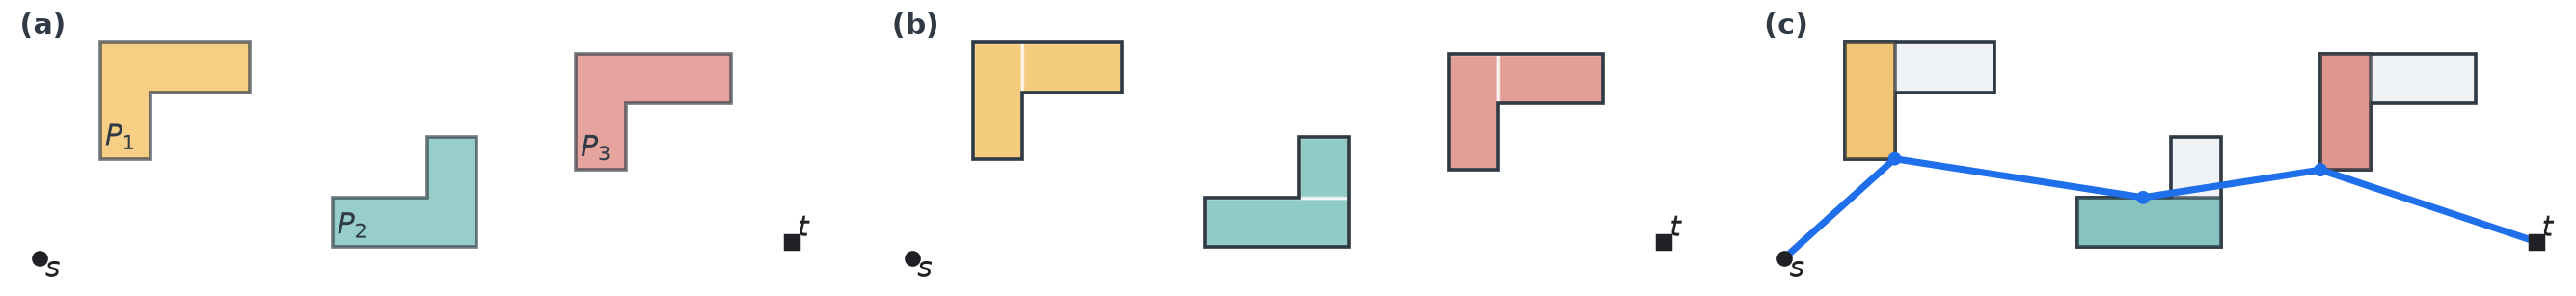
\includegraphics[width=0.96\textwidth]{assets/tpp-pipeline.pdf}\\[-0.20em]
	{\fontsize{8}{9}\selectfont Figura 1. Regiões não convexas, decomposição em peças convexas e solução do subproblema associado.}
\end{center}

\newpage

\begin{multicols}{2}

Na segunda camada, cada polígono não convexo é decomposto em peças convexas por uma implementação própria baseada no algoritmo de Greene [4], validada contra a rotina correspondente da CGAL em mais de 16 mil polígonos do conjunto de testes. O TPP não convexo é então resolvido por Branch and Bound: cada nó fixa uma escolha parcial de peças convexas, enquanto os polígonos ainda não fixados são relaxados por seus cascos convexos. Resolver exatamente esse problema relaxado fornece um limitante inferior. Se esse limitante excede o melhor caminho viável conhecido, toda a subárvore é descartada. Um incumbente inicial é obtido por uma heurística discreta sobre pontos representativos das fronteiras e refinado chamando o solver convexo nas peças selecionadas.

\section{Resultados}

A primeira contribuição do trabalho é uma implementação modular e verificável do TPP convexo, com separação entre primitivas geométricas, estruturas de consulta, espaços de trabalho reutilizáveis e ferramentas de benchmark. Os experimentos com instâncias sintéticas confirmam o comportamento assintótico esperado e mostram que a análise de pior caso não descreve completamente o desempenho observado: a estratégia memoizada reduz cálculos redundantes durante a reconstrução, enquanto a comparação com Tan e Jiang evidencia que a complexidade assintótica isolada não determina o desempenho prático.

A segunda contribuição é a redução efetiva do TPP não convexo com ordem fixa a uma busca controlada por limitantes geométricos. A enumeração direta das escolhas de peças é inviável. Em uma instância com 59 polígonos, por exemplo, a decomposição gera um espaço de busca da ordem de \(2\cdot10^{33}\) combinações. A versão atual do Branch and Bound resolve uma instância desse porte com cerca de 2 milhões de chamadas ao solver convexo, em aproximadamente 25 segundos, indicando uma redução de muitas ordens de grandeza no trabalho necessário para provar a otimalidade.

Além disso, foi construída uma infraestrutura de experimentação que registra chamadas ao solver convexo, nós visitados, nós podados, qualidade do incumbente, distribuição de peças e tempo gasto em cada etapa. Também foi desenvolvida uma visualização interativa para construir instâncias, inspecionar soluções e exibir mapas de último passo, facilitando a validação geométrica dos algoritmos.

\section{Conclusões}

O trabalho mostra que a combinação entre geometria computacional e otimização combinatória é uma abordagem promissora para o TPP não convexo. Em vez de formular todo o problema diretamente em um solver genérico, a estratégia proposta usa um algoritmo geométrico exato para resolver o subproblema convexo e o insere em uma árvore de Branch and Bound. Isso produz uma solução exata, reduz a dependência de solvers comerciais no núcleo do método e torna tratáveis instâncias que seriam impossíveis por enumeração direta.

Os próximos passos são fortalecer os limitantes, explorar decomposições convexas mais econômicas e estender a árvore de busca para também decidir a ordem de visita dos polígonos. Essa extensão conecta o projeto a variantes do Problema do Caixeiro Viajante com Vizinhanças e a modelos exatos de roteirização com regiões poligonais.

O autor declara não haver conflito de interesses.

O trabalho recebeu bolsa de Iniciação Científica da FAPESP, processo 2025/13861-1.

\section{Referências bibliográficas}

[1] M. Dror, A. Efrat, A. Lubiw, and J. S. B. Mitchell. Touring a sequence of polygons. \textit{Proceedings of the 35th Annual ACM Symposium on Theory of Computing}, 473-482, 2003.

[2] X. Tan and B. Jiang. Efficient algorithms for touring a sequence of convex polygons and related problems. \textit{Theory and Applications of Models of Computation}, 614-627, 2017.

[3] E. M. Arkin, S. P. Fekete, and J. S. B. Mitchell. The Traveling Salesman Problem with Neighborhoods: A Survey. In \textit{The Traveling Salesman Problem and Its Variations}, Springer, 2005.

[4] D. H. Greene. The decomposition of polygons into convex parts. In F. P. Preparata, editor, \textit{Computational Geometry}, 235-259, JAI Press, 1983.

[5] I. Gentilini, F. Margot, and K. Shimada. The travelling salesman problem with neighbourhoods: MINLP solution. \textit{Optimization Methods and Software}, 28(2):364-378, 2013.

\end{multicols}

\end{document}
